\documentclass[paper=a4, fontsize=11pt]{scrartcl}
\usepackage[left=25mm,top=30mm,right=25mm,bottom=30mm]{geometry}
\usepackage{titling}
\usepackage{dirtytalk}
\usepackage{mathtools}
\usepackage{multirow}
\DeclarePairedDelimiter{\ceil}{\lceil}{\rceil}
    
    \date{}
    \setlength{\droptitle}{-10em}
    \title{\textbf{Raport tema nr 3}}
    \author{Bucătaru Andreea A2 \and Bulboacă Maria A2}

\begin{document}

\maketitle
\section{Descrierea problemei}
\paragraph{}
Să se rezolve \textit{Problema comisului voiajor (TSP)} cu o metodă euristică și cu un algoritm genetic.

\section{Algoritmul utilizat}
\paragraph{}
Pentru rezolvarea acestei probleme, vom implementa un algoritm euristic și unul genetic. 
Acesta din urmă are la bază o strategie evolutivă, plecând de la o populație inițială de cromozomi care, 
pe măsură ce avansează, evoluează cu ajutorul operatorilor genetici. Doar cei mai puternici indivizi (cromozomi) vor supraviețui timp de mai multe generații.
\subparagraph{2.1}
Detalii de implementare pentru algoritmul genetic

\paragraph{}
Populația este reprezentată în memorie printr-o matrice care reține mai mulți cromozomi, fiecare cromozom fiind o listă de orașe (gene).

\underline{\smash{Inițializarea}} constă în crearea random a unor cromozomi. Generarea aleatoare a populației inițiale se face pe baza unei liste de orașe și distanțe date, interschimbând orașele între ele.

\underline{\smash{Funcția fitness}} este utilizată pentru a măsura calitatea cromozomilor. Ea este formulată plecând de la funcția numerică de optimizat. Trebuie să fie pozitivă și este construită pentru maximizare.
În cazul problemei noastre, valoarea fitness-ului pentru orașul $x$ va fi $1/y$, unde $y$ reprezintă costul distanței cromozomului $x$.

Scopul \underline{\smash{selecției}} este de a alege pentru supraviețuire cei mai adaptați indivizi din populație cu speranța că descendenții acestora vor avea un fitness mai ridicat.
O presiune de selecție ridicată duce la crearea unei diversități scăzute în populația creată.
Pe de altă parte, o presiune de selecție scazută încetinește evoluția.
În algoritmul implementat este folosită schema de selecție "Roata norocului".

\underline{\smash{Operatorii genetici}} folosiți sunt mutația (modificarea unei gene alese aleatoriu) 
și încrucișarea (schimbul de informație genetică între doi cromozomi).

\subparagraph{2.2}
Pseudocodul algoritmului genetic

\begin{enumerate}
    \itemsep0em
    \item[1.] Se generează random o populație inițială.
    \item[2.] Cât timp populația evoluează:
    \begin{enumerate}
        \item[a)] Se evaluează populația curentă.
        \item[b)] Se selectează cromozomii pentru următoarea generație.
        \item[c)] Cromozomii se supun încrucișării și mutației.
    \end{enumerate} 
    \item[3.] Se returnează cea mai bună soluție găsită.
\end{enumerate}

\subparagraph{2.3}
\textbf{Algoritmul euristic} folosește o abordare Greedy pentru a obține drumul de cost minim. 
Plecăm din fiecare oraș, alegând de fiecare dată cel mai apropiat oraș ,prin care nu am trecut, față de cel în care ne aflăm la un moment dat, 
iar când terminăm drumul curent comparăm cu cel mai bun găsit până acum. 

\subparagraph{2.4}
Pseudocodul algoritmului euristic
\begin{enumerate}
    \itemsep0em
    \item[1.] Se pornește din fiecare oraș.
    \item[2.] Cât timp mai sunt orașe nevizitate:
    \begin{enumerate}
        \item[a)] Se alege cel mai apropiat oraș, care nu a fost vizitat.
        \item[b)] Se compară cu cel mai bun drum găsit până atunci.
    \end{enumerate} 
    \item[3.] Se returnează cea mai bună soluție.
\end{enumerate}

\section{Rezultate experimentale}

\begin{table}[h]
    \resizebox{0.9\textwidth}{!}{\begin{tabular}{|l|l|l|l|l|l|l|}
    \hline
    Algoritm                 & Date de test & Nr orașe & Nr rulări           & Minim & Medie & Maxim \\ \hline
    \multirow{3}{*}{Genetic} & Djibouti     & 38       & \multirow{3}{*}{30} & 6693  & 8235  & 11510 \\ \cline{2-2}
                             & Berlin       & 52       &                     & 11919 & 13492 & 15637 \\ \cline{2-2}
                             & EIL          & 101      &                     & 2075  & 2289  & 2408  \\ \hline
    \end{tabular}}
    \end{table}


\begin{table}[h]
    \resizebox{0.8\textwidth}{!}{\begin{tabular}{|l|l|l|l|l|}
    \hline
    Algoritm                    & Date de test & Nr orașe & Nr rulări           & Rezultat \\ \hline
    \multirow{3}{*}{Euristic}   & Djibouti     & 38       & \multirow{3}{*}{1}  & 6770.08  \\ \cline{2-2}
                                & Berlin       & 52       &                     & 8182.19  \\ \cline{2-2}
                                & EIL          & 101      &                     & 736.36   \\ \hline
    \end{tabular}}
    \end{table}

\paragraph{}
Rezultatele algoritmului genetic au fost obținute cu o populație inițială de 1000 de cromozomi, 1000 generații,
$P\_CROSS = 0.05$ și $P\_MUTATION = 0.25$.

\underline{\smash{Influența valorilor parametrilor}}: Dacă mutația sau încrucișarea cromozomilor se realizează prea des, un individ nu poate evolua la fel de bine,
pentru că ar ajunge să fie complet diferit.
De asemenea, cu cât lăsăm populația să evolueze mai mult, cu atât o să obținem rezultate mai bune.

\begin{figure}[h!]
\begin{center}
    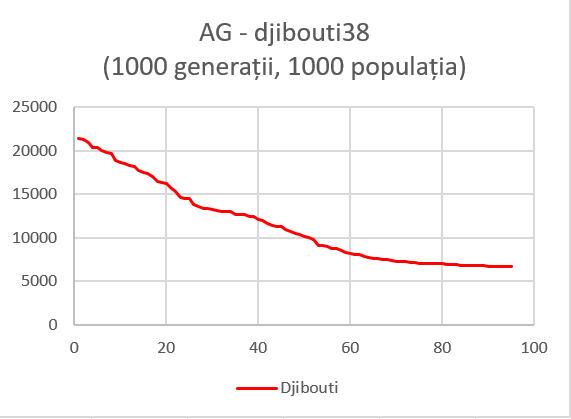
\includegraphics[scale=1]{Grafic_djibouti.png}
\end{center}
\end{figure}

\vspace{-17.8mm}
\begin{figure}[h!]
    \begin{center}
        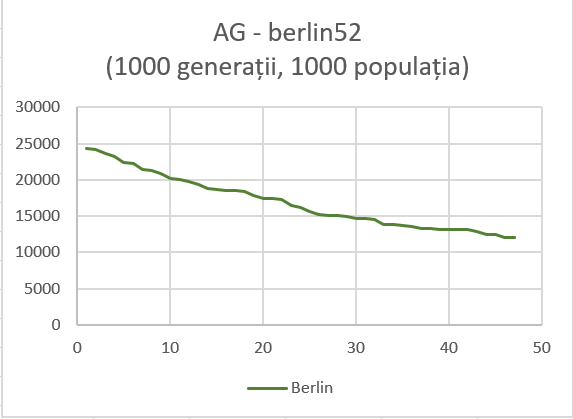
\includegraphics[scale=1]{Grafic_berlin.png}
        \vspace{200mm}
        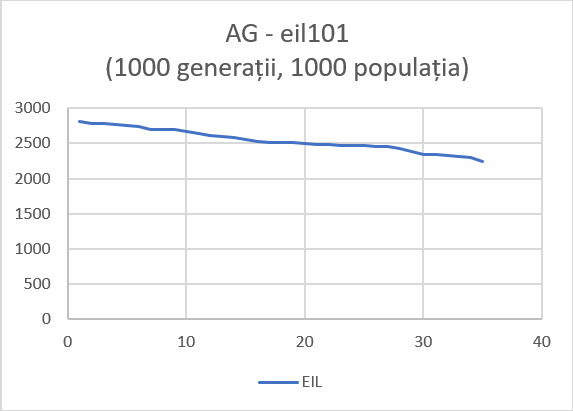
\includegraphics[scale=1]{Grafic_eil.png}
\end{center}
\end{figure}

\end{document}